\chapter{Who Do We Want To Come, Who Came?}

\section{Expanded Age Ranges}
Venturer Camps are traditionally held every three years. This cycle was disrupted by holding Common Ground International Camp in 2022, which was displaced from 2020 due to the Covid Pandemic. Not being able to hold a Venturer Camp in 2022, meant that there is one year's worth of Venturers who would have missed out on their Venturer Camp experience. For this reason, we decided to expand the age ranges of Venturer Camp 2023. The decision was made to include 16 and 17 year olds as Venturers. This would mean a small number of people who attended the 2019 camp as a participant would also be able to attend the 2023 camp as a participant.
\begin{figure}[h]
    \centering
    \begin{tikzpicture}
        \pie[text=pin]{48.9/13-15 y.o,
        17.3/16-17 y.o,
        33.8/18+
        }
    \end{tikzpicture}
    \caption{Booked attendees by age}
\end{figure}

By expanding the age ranges, we enabled more young people to participate in Venturer Camp 2023. We also enabled those 16 and 17 year olds who may never have experienced Woodcraft Folk outside their district or Common Ground, which was very structured, to have a looser structured Woodcraft Folk experience. The hope was that this would support them to transition to DFs, enabling them to grow their movement (the pandemic resulted in many DFs falling out of the movement). Figure \ref{fig:distribution-of-attendees} shows how some DFs were able to take on Volunteering roles as under-18 volunteers.
\begin{figure}[ht]
    \centering
    \begin{tikzpicture}
        \pie[text=pin]{65/Participant,
        1.11/U18 Volunteer,
        34/Volunteer
        }
    \end{tikzpicture}
    \label{fig:distribution-of-attendees}
    \caption{Distribution of Attendees}
\end{figure}

\section{International Delegations}
In Autumn 2022 we were also hoping that we would be able to support a number of international delegations to attend. We discussed a number of models through which we could facilitate this with a very small coordination team. The majority favoured being that a group or district would be responsible for all aspects of supporting an international delegation.\\

In Spring 2023, the general enquiries inbox was contacted about the possibility of hosting a group from an English Language school situated in Spain. However, due to the Woodcraft knowledge barrier and the implied expectation that we (the central coordination team) would be responsible for supporting this group to attend, the decision was made to decline this request. At this time, the coordination team was stretched very thinly, with many people taking on more than what they'd expected to be doing in the run up to the event.\\

We were, unfortunately, unable to host any international delegations at Venturer Camp 2023. 

\section{Centrally Organised Equipment}
During the conceptualisation of Venturer Camp 2023, we decided that to reduce burdens on Villages - we would centrally organise the equipment which was being assigned to Villages. This concept, what worked well and what didn't work about it will be explored in the Site Services \& Production Team's section - there are very mixed views about this!


\begin{figure}[ht]
    \centering
    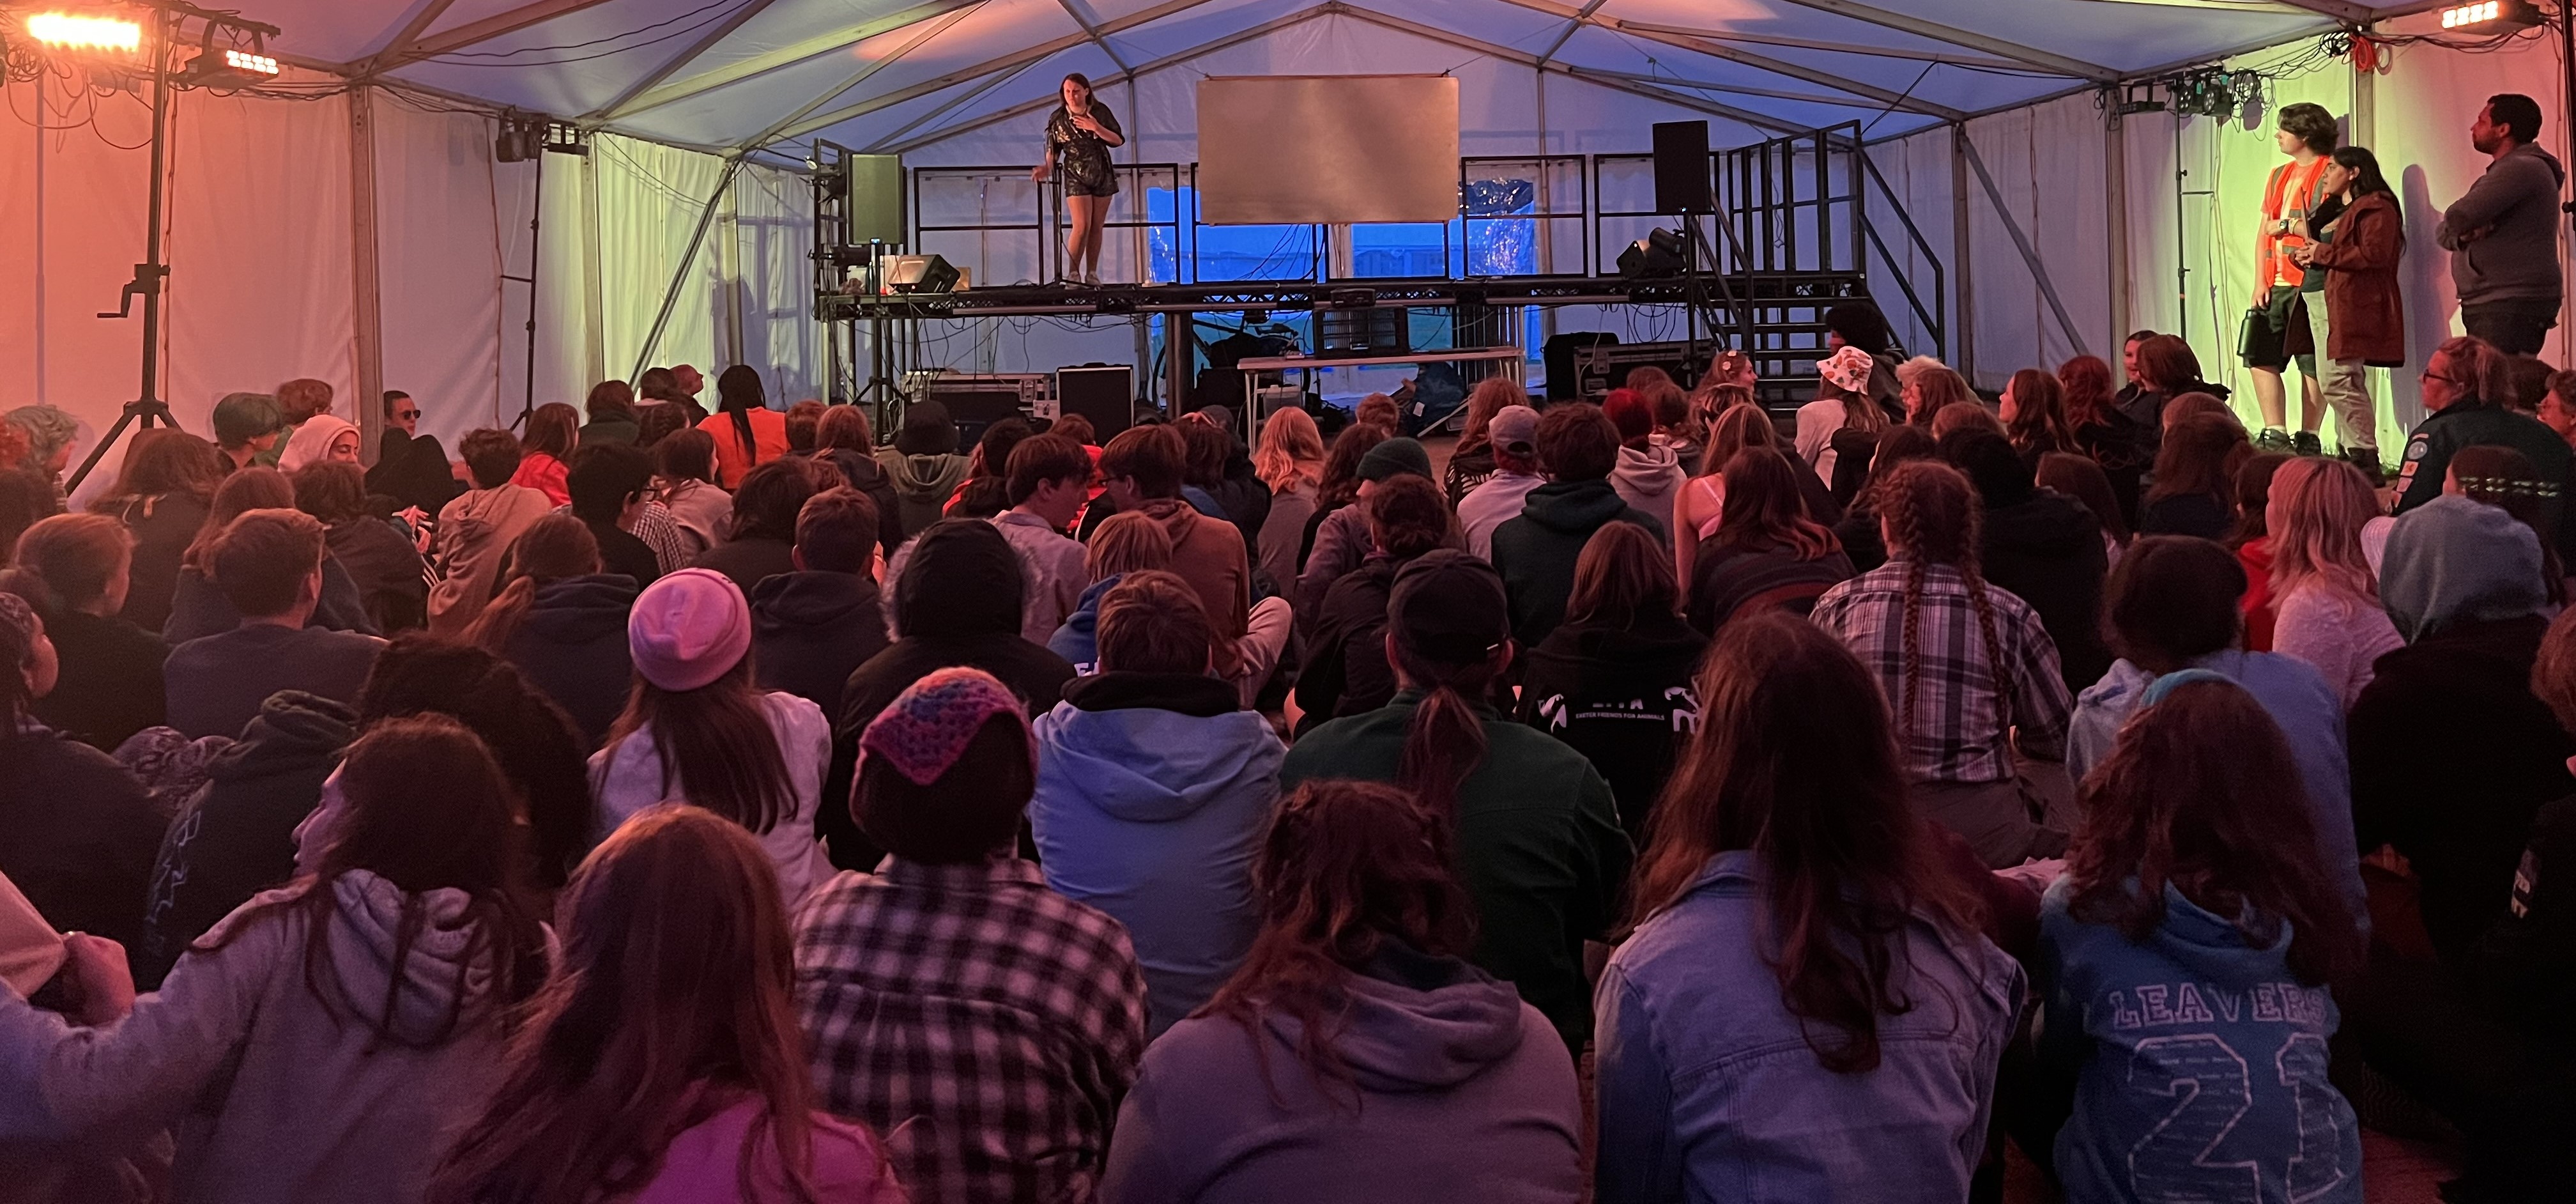
\includegraphics[width=0.8\textwidth]{assets/opening-night-ab.jpeg}
    \caption{Opening Night Performance (\textit{AB})}
\end{figure}